\section{Cyfrowy algorytm PID i DMC}

\subsection{Algorytm PID}

Regulator PID to regulator składający się z 3 członów:\newline
\indent- proporcjonalnego P o wzmocnieniu $K_{r}$, kompensuje uchyb
bieżący\newline
\indent- całkującego I o czasie zdwojenia $T_{i}$, kompensuje akumulację
uchybów z przeszłości\newline
\indent- różniczkującego D o czasie wyprzedzania $T_{d}$, kompensuje
przewidywane uchyby w przyszłości\newline

Ważona suma tych trzech działań stanowi podstawę sygnału
podawanego na człon wykonawczy w celu regulacji procesu (np.
zmiana położenia zaworu regulacyjnego albo zwiększenie mocy
grzałki).
Regulator realizuje algorytm:
$$u(t) = Kr\Bigg(e(t)+\int e(\tau)d\tau+T_{d}\frac{de(t)}{dt}\Bigg)$$
gdzie $u(t)$ - sygnał wyjścia regulatora, $e(t)$ - uchyb regulacji.

Transmitancja regulatora PID
$$G(s) = K_{r}\Bigg( 1 +\frac{1}{T_{i}s}+T_{d}s\Bigg)$$
W realizacji naszego zadania wykorzystany był dyskretny regulator PID.
Sterowanie regulatora wyznaczane było z poniższych wzorów, które
zostały otrzymane dzięki metodzie Eulera i całkowania metodą
trapezów:

$$u(k)=u_{P}(k)+u_{I}(k)+u_{D}(k)$$

\indent gdzie
$$u_{P}(k)=K_{r}e(k)$$
$$u_{I}(k)=u_{I}(k-1)+\frac{K_{r}}{T_{I}}T_{p}\frac{e(k-1)+e(k)}{2}$$
$$u_{D}=K_{r}T_{D}\frac{e(k)-e(k-1)}{T_{p}}$$


\subsection{Algorytm DMC}

Algorytm DMC (Dynamic Matrix Control) algorytm regulacji predykcyjnej. 
Do predykcji wykorzystuje się model procesu w postaci odpowiedzi skokowych. 
W algorytmie DMC dynamika obiektu regulacji modelowana jest dyskretnymi odpowiedziami skokowymi, 
które opisują reakcję wyjścia na skok jednostkowy sygnału sterującego.
 
\begin{figure}[H]
    \centering
    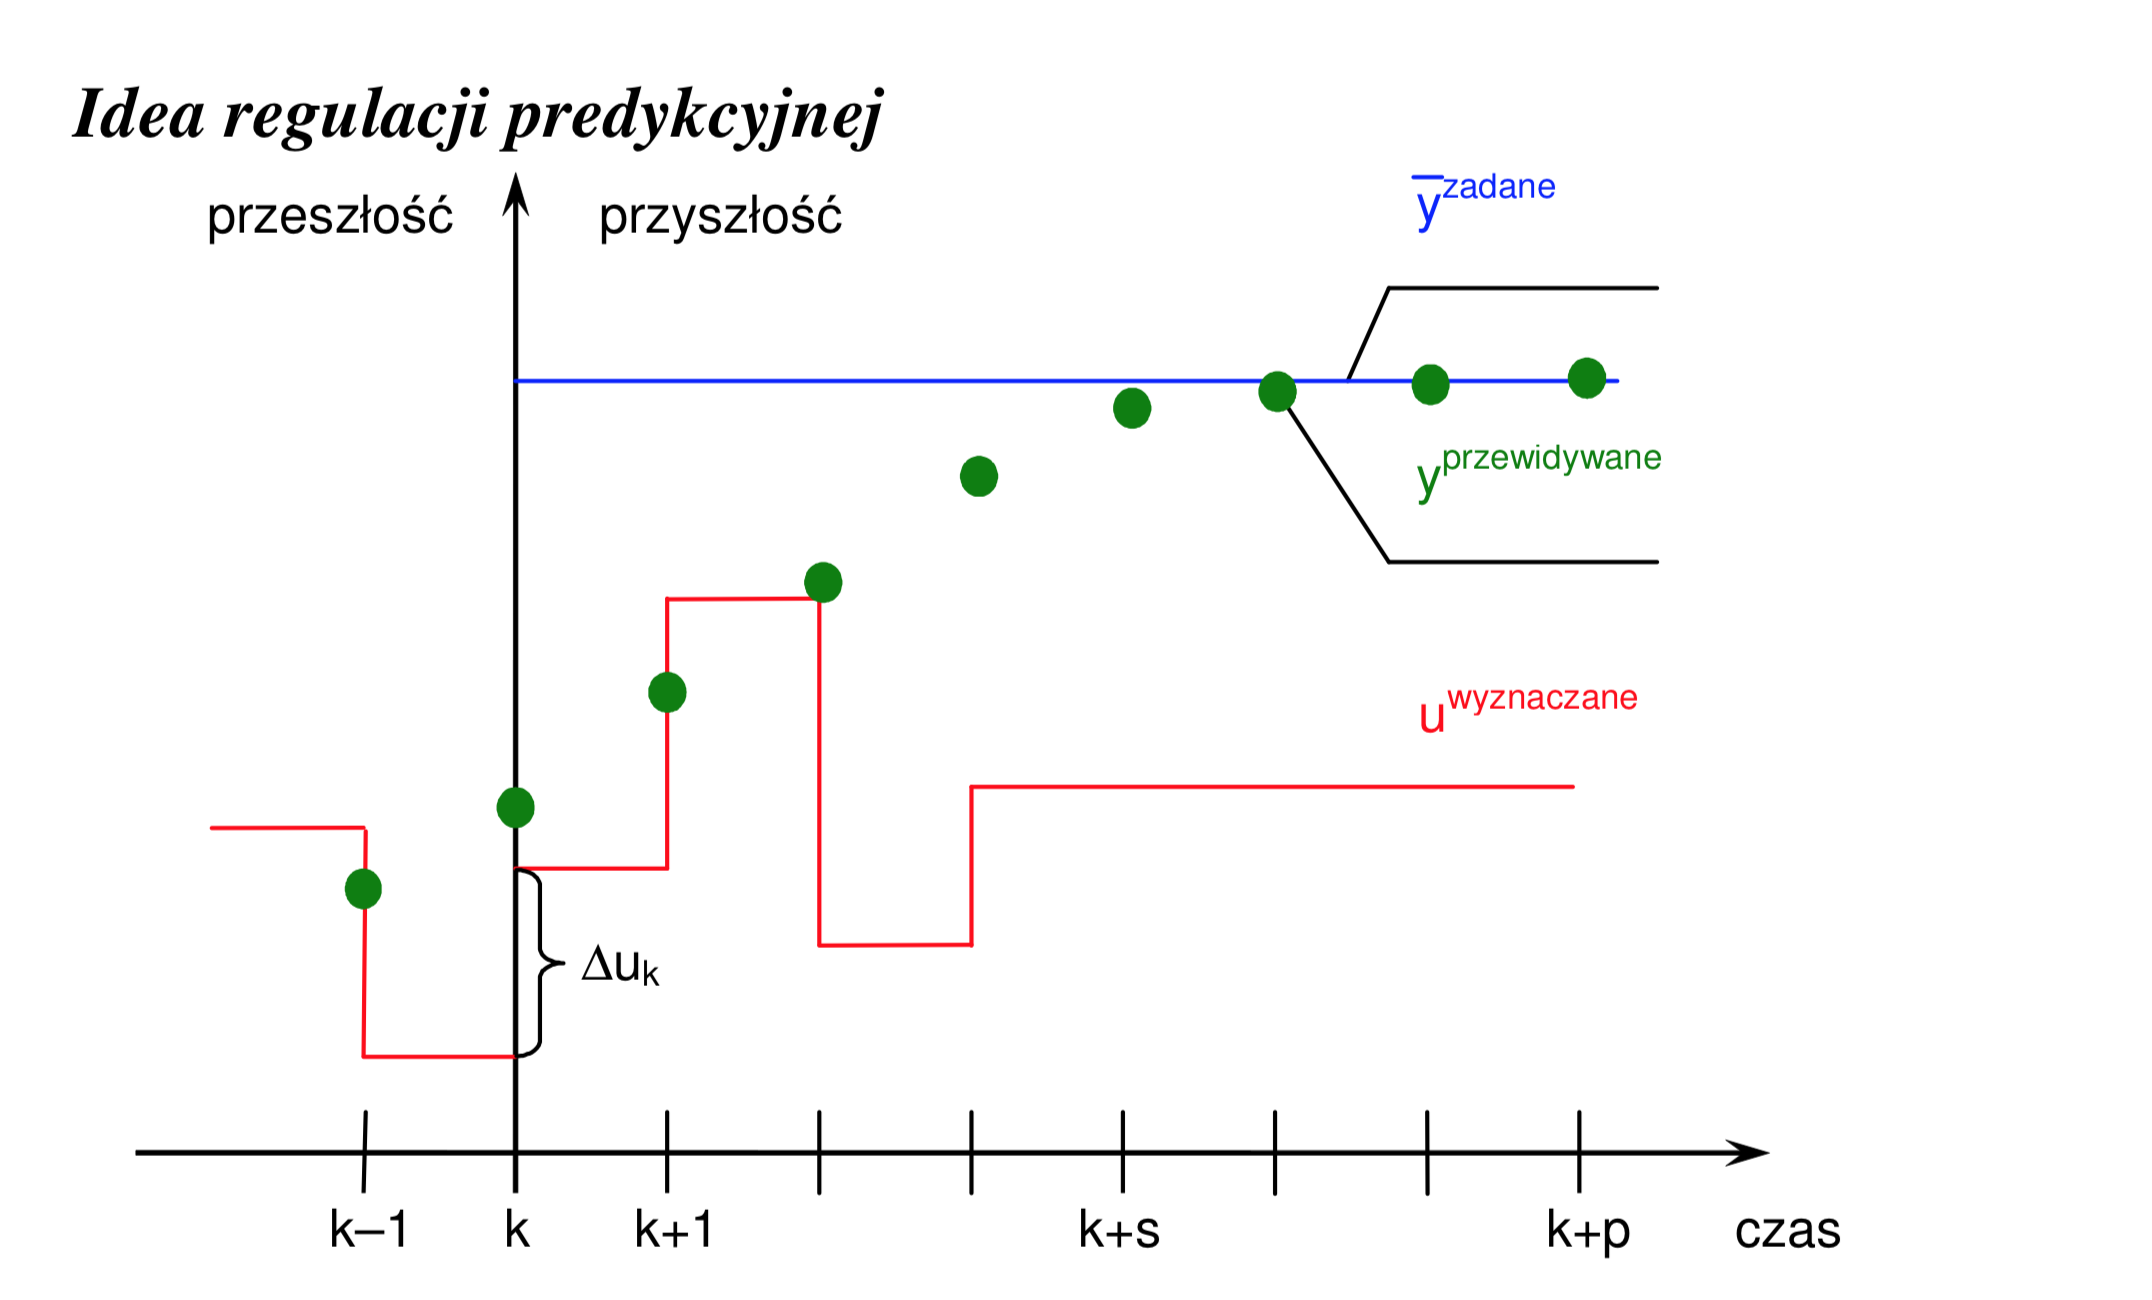
\includegraphics[scale=0.25]{dmc_idea.png}
    \caption{Idea działania regulatora DMC}
\end{figure}
